\section{FlipFlop Calculus With  $\mathcal{LR}$ Refinement} \label{sec:flip-flop}
% in case this will be added at some point
%
%
%

\kasten{
\subsubsection*{FlipFlop calculus (FFC) overview}
\begin{calcfeatures}
	\feature{calculus identifier}{ffc, ff, flipflop}
	\feature{calculus parameters}{none}
	\feature{arity}{ternary}
	\feature{entity type}{2D points}
	\feature{description}{relates the referent $C$ relative to the line segment starting at origin $A$ and ending at relatum $B$ resulting in nine base relations}
	\feature{base relations}{l (left), r (right), f (front), b (back), i (inside), s (start), e (end), dou, tri}
	\feature{references}{\citet{Ligozat93_FlipFlopCalculus,scivos:nebel:icsc-04}}
        \lastfeature{remark}{\engine{} uses the $\mathcal{LR}$ refinement in its implementation of the FFC}
\end{calcfeatures}
}

The FlipFlop calculus proposed in \citet{Ligozat93_FlipFlopCalculus}
describes the position of a
point $C$ (the referent) in the plane with respect to two other points
$A$ (the origin) and B (the relatum) as illustrated in Fig.
\ref{fig:FFC}. It can for instance be used to describe the spatial
relation of $C$ to $B$ as seen from $A$. For configurations with $A\neq B
$ the following base relations are distinguished: $C$ can be to the
\textbf{l}eft or to the \textbf{r}ight of the oriented line going
through $A$ and $B$, or $C$ can be placed on the line resulting in one of
the five relations \textbf{i}nside, \textbf{f}ront, \textbf{b}ack,
\textbf{s}tart ($C = A$) or \textbf{e}nd ($C = B$) (cp. Fig.
\ref{fig:FFC}). Relations for the case where $A$ and $B$ coincide were
not included in Ligozat's original definition
\citep{Ligozat93_FlipFlopCalculus}. This was done with the $\mathcal{LR}$
refinement \citep{scivos:nebel:icsc-04} that introduces the relations
\textbf{dou} ($A=B \neq C$) and \textbf{tri} ($A=B=C$) as additional
relations, resulting in 9 base relations overall. A $\mathcal{LR}$ relation $rel_\mathcal{LR}$
is written as $A,B\; rel_\mathcal{LR}\; C$, e.g. $A,B\; \textbf{r}\; C$ as depicted in Fig.~\ref{fig:FFC}.


\begin{figure}[htp]
	\centering
	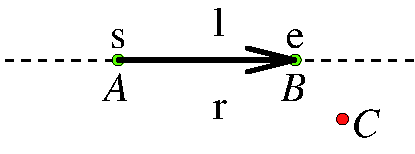
\includegraphics[width=0.4\textwidth]{flipflop_basenew}
	\caption{The reference frame for the $\mathcal{LR}$ calculus, an enhanced version
		 of the FlipFlop Calculus}
	\label{fig:FFC}
\end{figure}
